%%%%%%%%%%%%%%%%%%%%%%%%%
% Dokumentinformationen %
%%%%%%%%%%%%%%%%%%%%%%%%%
\include{revision}
\newcommand{\titleinfo}{Wissensbasierte Systeme - Formelsammlung}
\newcommand{\authorinfo}{R. Nestler}
\newcommand{\versioninfo}{$Revision: \revision$ - powered by \LaTeX}

%%%%%%%%%%%%%%%%%%%%%%%%%%%%%%%%%%%%%%%%%%%%%
% Standard projektübergreifender Header für
% - Makros 
% - Farben
% - Mathematische Operatoren 
%
% DORT NUR ERGÄNZEN, NICHTS LÖSCHEN
%%%%%%%%%%%%%%%%%%%%%%%%%%%%%%%%%%%%%%%%%%%%%  
\include{header/header}

\renewcommand{\arraystretch}{1.0}

\usepackage{tikz}
\usepackage{enumitem}
\usepackage{tabularx}
\usepackage[compact]{titlesec}
\usepackage[belowskip=-10pt,aboveskip=0pt]{caption}
\titlespacing{\section}{0pt}{*0}{*0}
%\titlespacing{\subsection}{0pt}{*0}{*0}
\titlespacing{\subsubsection}{0pt}{*0}{*0}

%\setlength{\headsep}{2pt}

%\parskip 0pt

\setlist{nosep}

\lstset{
	tabsize=2,
	language=Mathematica,
	basicstyle=\footnotesize\sffamily,
	keywordstyle=\color[rgb]{0,0,1},
	commentstyle=\color[rgb]{0.133,0.545,0.133},
	stringstyle=\color[rgb]{0.627,0.126,0.941}
}

% Möglichst keine Ergänzungen hier, sondern in header.tex
\begin{document} 

\section{Mathematica}
\begin{table}[!h]
	\begin{tabularx}{\textwidth}{p{6cm} X}
		Back Propagation mit einer versteckten Schicht Fehler mit Kettenregel &
		\vspace{-5mm}
		\lstinputlisting{listings/backPrp1Hid.mm} \\
		Diskretes Hopfield Netzwerk mit Energiefunktion &
		\vspace{-5mm}
		\lstinputlisting{listings/hopfield.mm}
	\end{tabularx}
	\caption{Verschiedene Mathematica Code-Auszüge}
	\label{tab:mathematica}
\end{table}


\section{Optimierung}
\subsection{Graphische Methoden}
\subsubsection{Sprague Grundy}
\begin{tabularx}{\textwidth}{XX}
	\vspace{-4cm}
\begin{enumerate}
	\item Endknoten (Verlierpositionen) haben Rang 0
	\item Von jeder Gewinnerposition führt mind. ein Pfeil auf einen Rang 0 Knoten
	\item Alle Pfeile von einem Knoten mit Rang 0 führen zu einem Knoten mit Rang $>$ 0
\end{enumerate} &
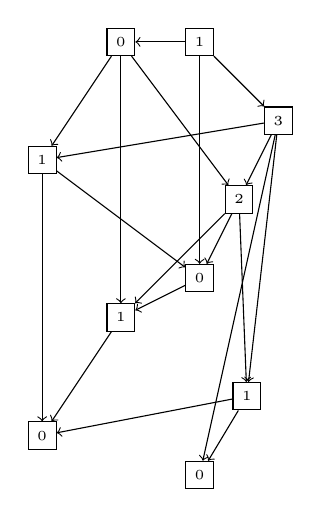
\begin{tikzpicture}[font=\tiny]
	\node (a) at (1,0) [draw]{0};
	\node (b) at (2,0) [draw]{1};
	\node (c) at (3,-1) [draw]{3};
	\node (d) at (0,-1.5) [draw]{1};
	\node (e) at (2.5,-2) [draw]{2};
	\node (f) at (2,-3) [draw]{0};
	\node (g) at (1,-3.5) [draw]{1};
	\node (h) at (2.6,-4.5) [draw]{1};
	\node (i) at (0,-5) [draw]{0};
	\node (j) at (2,-5.5) [draw]{0};

	\draw[->] (a)--(d);
	\draw[->] (a)--(e);
	\draw[->] (a)--(g);

	\draw[->] (b)--(a);
	\draw[->] (b)--(c);
	\draw[->] (b)--(f);

	\draw[->] (c)--(d);
	\draw[->] (c)--(e);
	\draw[->] (c)--(h);
	\draw[->] (c)--(j);

	\draw[->] (d)--(f);
	\draw[->] (d)--(i);

	\draw[->] (e) -- (h);
	\draw[->] (e) -- (f);
	\draw[->] (e) -- (g);

	\draw[->] (f) -- (g);

	\draw[->] (g) -- (i);

	\draw[->] (h) -- (i);
	\draw[->] (h) -- (j);
\end{tikzpicture}
\end{tabularx}

\subsection{Lagrange}
Lagrange Multiplikatoren definieren Nebenbedingungen:\\
\begin{tabular}{l l l}
	{$ h(x,\lambda) = f + \sum\limits_{k=1}^s{\lambda_k g_k} $ } &
		$s$:    &Anzahl Nebenbedingungen \\
		&$f(x)$:&Zu optimierende Funktion \\
		&$g_k$: &Nebenbedingungen mit $g_k(x) = 0$
\end{tabular}
\subsubsection{Beispiel}
Auf der Funktion $f(x,y) = x^2 + y^2$ ist der tiefste Punkt zu finden,
für den gilt: $y = 3x - 5$ \\
$ h(x,y,\lambda) = x^2 + y^2 + \lambda(y - 3x + 5) $ \\
Partielle Ableitungen $h'(x,y,\lambda)$ Null setzen
\begin{tabular}{ll}
	$f'(x)$&$ = 2 x + 3 \lambda$ \\
	$f'(y)$&$ = 2 y + \lambda$ \\
	$f'(\lambda)$&$ = y - 3x + 5$
\end{tabular}

Dieses Gleichungssystem kann dann ganz normal aufgelöst werden.

\subsection{Lineare Optimierung}
\subsubsection{Gradientenabstieg} \label{2_Gradientenabstieg}
\begin{enumerate}
	\item Startpunkt wählen
	\item Entlang des steilsten Abstiegs entlang bis Steigung zunimmt
	\item Neu ausrichten und wiederholen
	\item Fertig wenn Gradient nach unten zeigt
\end{enumerate}
Der Gradientenabstieg kann nur funktionieren wenn es keine lokalen
Minimas gibt. Existieren lokale Minimas muss ``gerüttelt'' werden, um
aus dem lokalen Minima auszubrechen.
Das Lernen eines Perzeptrons entspricht einem Gradientenabstieg

\section{Neuronale Netze}
Ein Neuron ist ein Schwingkreis. Es hat n Eingänge und einen Ausgang. Die Werte der
Eingänge werden summiert. Wenn die Summe der Eingänge einen Schwellwert übertrifft, wechselt der Ausgang, das Neuron feuert.
Für die Schwellwertfunktion, wird entweder die Signum (0/1) oder die Sigmoid-Funktion welche ``weiche'' Kanten hat und ableitbar ist verwendet.
\begin{figure}[htb]
	\centering
	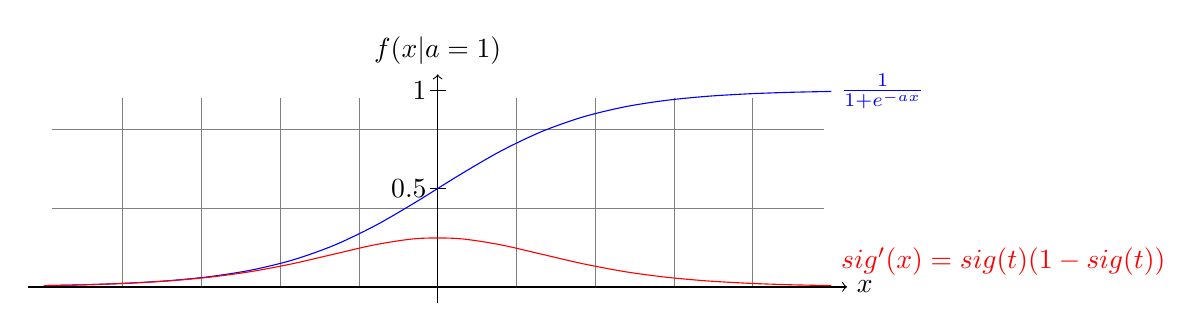
\begin{tikzpicture}[domain=-5:5, smooth, samples=20]
	\draw[very thin, color=gray] (-4.9,0.0) grid (4.9,2.4);

	\draw[->] (-5.2,0) -- (5.2,0) node[right] {$x$};
	\draw[->] (0,-0.2) -- (0,2.7) node[above] {$f(x|a=1)$};
	\draw (-0.1,2.5) --(0.1,2.5) node [left] {$1~$};
	\draw (-0.1,1.25) -- (0.1,1.25) node [left] {$0.5~$};

	\draw[color=blue] plot (\x,{2.5 / (1+exp(-\x))}) node[right] {$\frac{1}{1+e^{-ax}}$};
	\draw[color=red]  plot (\x,{2.5 / (1+exp(-\x)) * (1-1/(1+exp(-\x)))}) node[above right] {$sig'(x)=sig(t)(1-sig(t))$};
\end{tikzpicture}


	\caption{Sigmoid Funktion mit a=1}
\end{figure}
\newpage
\subsection{Übersicht}
\begin{table}[htbp]
	\centering
	\begin{tabular}{l | p{8cm}}
		Typ & Merkmale \\
		\hline
		{klassisches Perzeptron} & {
			\begin{itemize}
				\item Können nur linear separierbare Probleme lösen
				\item Ein einzelnes Perzeptron-Neuron kann 14 Schnittebenen legen
			\end{itemize}
		}
		\\
		{Holographisches Perzeptron} & {
			\begin{itemize}
				\item Verwendet Komplexe Zahlen
				\item Sehr grosse Speicherfähigkeit
				\item Grosse Verarbeitungsgeschwindigkeit
				\item Stochastische Resonanz (benötigt Rauschen im Input)
			\end{itemize}
		}
		\\
		{Kohonen-Netze} & {
			\begin{itemize}
				\item Topographisches Netz
				\item Geeignet für TSP-Problem
			\end{itemize}
		}
		\\
		{Hopfield} & {
			\begin{itemize}
				\item Lernt nicht bzw. unüberwachtes Lernen
				\item Nur eine Schicht, gleichzeitig Ein- und Ausgabe
				\item Jedes der binären Neuronen mit jedem verbunden
				\item Erkennt invertierte Muster als gleich
			\end{itemize}
		}
	\end{tabular}
	\caption{Vergleich zwischen verschiedenen Neuronalen Netzen}
	\label{tab:nnetze}
\end{table}
\subsection{Klassisches Neuron / Perzeptron}
Das Perzeptron ist das klassische mathematische Neuron. Es besteht aus:
\begin{itemize}
	\item Summierer
	\item Feuerschwelle
	\item Ausgabefunktion (Sigmoid)
\end{itemize}
\subsection{Netze elementarer Perzeptronen}
\subsection{Backpropagation}
\subsection{Holographisches Perzeptron}
\subsection{Kohonennetze}
\subsection{Hopfield}
Das Hopfield-Netz ist geeignet um Muster (Bilder) zu kennen. Dabei wird pro Pixel ein binäres Neuron verwendet (-1,1).
Dazu erstellt man eine Korrelationsmatrix, welche alle Muster enthält, es wird nicht gelernt!
Pro zu erkennendes Muster werden etwa 7 Neuronen benötigt.
Für eine gute Erkennung sollten die Muster möglichst orthogonal, also linear unabhängig sein.


\section{Genetische Algorithmen}
Genetische Algorithmen gründen auf der Formalisierung der wichtigsten
Prozesse und Begriffe aus der Evolution:
\begin{itemize}
	\item Kreuzung
	\item Mutation
	\item Fitness
\end{itemize}
Keine Muster für Zuordnung, dafür Funktionen und eine Fitnesslandschaft.
Die Fitnesslandschaft ersetzt die Korrelationsmatrix des
Hopfield-Netzwerks.
\subsection{Ablauf}
\begin{enumerate}
	\item Zufällige Chromosomen erstellen
	\item Gemäss Fitness Wahrscheinlichkeit für nächste Kreuzung bestimmen
	\item Zwei Chromosomen mit skalierter Wahrscheinlichkeit auswählen
		und an zufälliger Stelle teilen und je mit dem anderen
		Gegenstück zusammensetzen.
	\item Die neu erstellten Chromosomen dürfen leicht mutiert werden.
\end{enumerate}
\subsection{Genetische Programmierung}
Anwendung von genetischen Algorithmen auf Programme selbst, bei denen
der Zweck definiert ist. Die Fitnessfunktion entspricht dabei dem
Erfüllen der Aufgabe.


\section{Clustering}
\subsection{Übersicht}
\usetikzlibrary{trees}
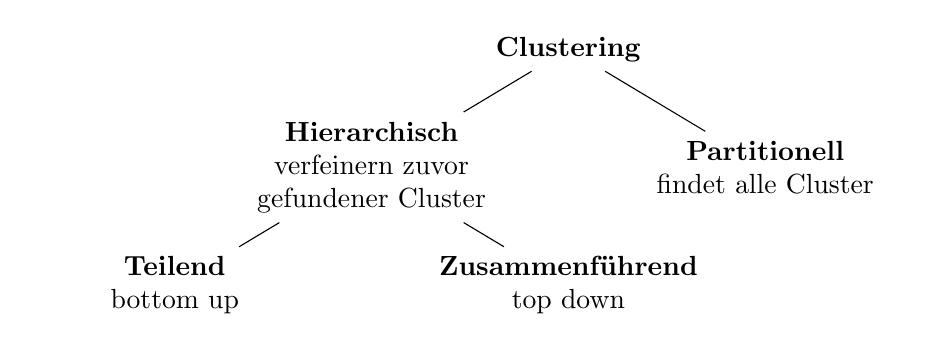
\begin{tikzpicture}[
	text width=3.5cm, align=flush center,
	level 1/.style={level distance=1.5cm, sibling distance=5cm},
	level 2/.style={}
]
	\node {\textbf{Clustering}}  % root {
		child { node {\textbf{Hierarchisch}\\verfeinern zuvor gefundener Cluster}
			child {node {\textbf{Teilend}\\ bottom up}}
			child {node {\textbf{Zusammenführend}\\ top down}}
		}
		child { node {\textbf{Partitionell} \\ findet alle Cluster} }
	;
\end{tikzpicture}

\subsection{Distanzmasse}
Bevor man überhaupt clustern kann, benötigt man eine passende Distanzfunktion für die einzelnen Elemente untereinander und zu einem Cluster.
\begin{table}[htbp]
	\centering
	\begin{tabular}{p{8cm} | p{8cm}}
		Beschreibung & Formel \\
		\hline
		{Der minimale/maximale Abstand} & {
			$\underset{a \in A, b \in B}{min}\{d(a,b)\} ~ \underset{a \in A, b \in B}{max}\{d(a,b)\}$
		}
		\\
		{Der durchschnittliche Abstand aller Elementpaare aus den beiden Clustern (average linkage clustering)} & {
			$\frac{1}{|A||B|} \sum\limits_{a \in A, b \in B}{d(a,b)}$
		}
		\\
		{Der durchschnittliche Abstand aller Elementpaare aus der Vereinigung von A und B} & {
			$\frac{1}{|C|} \sum\limits_{x,y \in C, C=A \cup B}{d(x,y)}$
		}
		\\
		{Der Abstand der Mittelwerte der beiden Cluster} & {
			$d(\overline a, \overline b)$
		}
		\\
		{Die Zunahme der Varianz beim Vereinigen von A und B (Wards method)} & {
			$\frac{\overline a, \overline b}{\frac{1}{|A|} + \frac{1}{|B|}}$
		}
	\end{tabular}
	\caption{Verschiedene Distanzmasse}
	\label{tab:distanzmasse}
\end{table}
\subsection{K-means Clustering}
Unüberwachtes hartes Clusteringverfahren welches nicht unbedingt konvergiert.
\subsection{SCC- / Pott-Spin Clustering}
Es wird nicht vorgegeben wieviel Cluster erwartet werden. Pott-Spin verwendet Temperatur, SCS kann Cluster unterschiedlicher Dichte aufspüren.


 
\end{document}
